\documentclass{article}
    \title{Thesis Proposal: Garden of Eden}
    \author{William B. Jackson}
    \date{February 5, 2014}

    \newcommand{\tab}{\hspace*{2em}}
    \usepackage{fullpage}
    \usepackage{alltt}
    \usepackage{natbib}
    \usepackage{graphicx}

\begin{document}
    \maketitle
    \section{(really bad) Abstract} % NOTE: this is really bad and needs to be re-written.
    \tab Garden of Eden (GoE) is an exercise in procedural generation of lifelike worlds. Using
parallelized computations, it randomly generates a forest scene of realistically shaped and
proportioned asymmetric trees on top of a basic topographical map. This map is then rendered in 3D,
with support for user navigation. The end result of this project is a sort of game: a static
rendering of a natural environment, exploring how humans find visual pleasure and meaning in virtual
environments. The passive interaction of the user is vital to this simulation, as it reflects how
one would observe a natural environment; ideally, the simulation would evoke similar reactions to
the environment GoE seeks to emulate, thus exploring the concept of a “natural”, the distinction
between real and virtual, and one's own sense of place.
 
    % Intro: what is the need? motivation, difficulty, etc.
    % Abs: ad for the paper, shorter,  mirrors introduction, fewer results and motivation
    % Refocus on engineering

    \section{Related Work}
        % Phrase any assertions with relation to thesis as things done
        % Phrase tentatively if I didn't do it
    \tab A significant body of work relating to natural feature generation exists in the video game
industry. Minecraft\cite{minecraft}, for example, uses advanced terrain and feature generation
techniques to procedurally create such natural features as mountain ranges, cave systems, chasms,
coasts, and flora biomes, as well as artifical features such as temples, villages, and mine shafts.
It achieves truely impressive scenes using simplified graphics, resulting in a stylised look rather
than striving for verisimillitude. Another game worth mentioning in this context is
Proteus\cite{proteus}, a small-scale "game of audio-visual exploration and discovery" that allows
users to explore a highly-stylized generated island. There are many other games that use feature
generation techniques, either as the creative force of the game world or to fill in between created
features; I mention these two primarily because, through both gameplay and simple, yet awesome,
natural scenery, they served as inspiration for this project.

    % Computer rendering of stochastic models
    % Diffusion equation
    % Mandelbrot FBR
    % Eroded fractal terrain
    % Terrain gen with genetic algorithms
    % Mighty maple
    % Plant automata
    % Plant models

    \section{Terrain}
        \subsection{Midpoint Displacement}
    \tab The Midpoint Displacement algorithm, also known as the Diamond-Square algorithm, is an easy
way to generate surface height maps for terrain. The algorithm is as follows\cite{martz97}:
    \begin{verbatim}
Loop while quadrilateral side is at least 1
    // Square step
    For each discrete square of given quadrilateral side length
        Get midpoint of square
        Calculate random offset as a random number in a specified range times a scale
        Midpoint becomes average of square's corners plus random offset

    // Diamond step
    For each discrete diamond defined by the square step's calculated midpoints
        Get midpoint of diamond
        Calculate random offset as a random number in a specified range times a scale
        Midpoint becomes average of diamond's corners plus random offset

    Decrease scale by a constant fraction
    Half quadrilateral side

    \end{verbatim}

    % Discuss testing
    % Look at paper, look at actual terrain for constants
    % Discuss size scale
    % GIS data?

    \tab The algorithm is works well to generate fractal surfaces, and allows for a decent amount
of control over the percieved "roughness" of the resultant surface in how one defines the scale
factor. However, it is fairly slow, and there are also well-documented artifacts, notably for
steeper surfaces. These factors can be mitigated somewhat with careful selection of constants,
discussed below.

        \subsection{Feature Extraction}

        \subsection{Gaussian Filter}

    \section{Trees}
        \subsection{L-Systems}
    \tab An L-System, as defined in \cite{abp96} describes a recursive substitution system to
build increasingly complex strings. A system consists of an initial value or set of values, and a
series of rules used to recursively replace sections of the initial set. The set consists of
productions, or operations that, when combined with a rule, represent a certain kind of predictable
growth. Productions can, for example, represent a single branching structure, or trunk growth. As
such, L-Systems are an excellent way to represent the growth of trees, as they give a simple "seed"
rules by which it can branch in a biologically feasable way into a much larger system. As L-Systems
consist of self-replacement rules, they tend to form fractal systems, which are "self-similar" at
different levels of detail. In an L-System, this self-similarity at smaller levels of detail comes
from the recursion depth, which replaces productions at small levels with smaller versions of the
designs seen at a larger scale.


            \subsubsection{Productions}
    \tab A production defines a particular recursive structure. In combination with its replacement
rule, it acts similarly to a replacement function; a single production can be replaced by a set of
other productions, including itself, leading to interesting fractal shapes. In this project, a
production does not represent any physical shape, and is not drawn graphically; instead, it's 
replacement rule can contain graphical information, allowing a production to represent a specific
physical occurance. A production can, for example, represent a bijunction branching, or a bending
of a branch due to biological influences, or the thickening of the trunk due to age.

            \subsubsection{Parametric L-Systems}
    \tab A parametric L-System contains parametric productions, or, more simply, producitons that
take parameters. Production rules change to accomidate parameter logic, matching, for example, only
if a production has a "time" greater than 5. In this way, productions representing specific growth
actions can have significantly different geometry while still having the same basic structure. A
branch production, for example, might take an angle parameter, which would make larger branches
diverge less dramaticaly than twigs.

    \tab The below L-System can serve as an example, and is used as the L-System module's tester in
\verb|./test/lsys\_console.html|.
    % This is broken
    \begin{alltt}
    \(\omega\)  : B(2)A(4,4)
    \(p\sb{1}\) : A(x,y) : \(y \leq 3 \rightarrow\) A(x*2, x+y)
    \(p\sb{2}\) : A(x,y) : \(y > 3 \rightarrow\) B(x)A(x/y, 0)
    \(p\sb{3}\) : B(x)   : \(x < 1  \rightarrow\) C
    \(p\sb{4}\) : B(x)   : \(x \geq 1 \rightarrow\) B(x-1)   
    \end{alltt}
In this example, $\omega$ gives the initial productions with parametric values. The rules have
changed both to check the values of the parameters, and replace accordingly, and to modify the
parameters in the replacement step. In this way, the productions will have different parameters at
each level of recursion, reflecting changing growth at more depth.

            \subsubsection{Turtle Graphics}
    \tab As stated before, productions give no graphical information as to how a tree is drawn.
Thus, in addition to productions, an L-System must implement a system of graphical information. In
order to create branching structures, LOGO-style turtle graphics are used to draw on the HTML5
canvas. Invented as a simple graphics drawer for educational purposes, turtle graphics consist of a
set of commands that direct the movement of a "turtle", or a drawing point. In 3D space, three
dimensions of orientation are controlled by issuing commands with a specified radial change;
drawing occurs by moving the turtle forward. The turtle commands implemented are as follows:

\begin{center}
\begin{tabular}{|l|l|l|p{7cm}|}
    \hline
    Command & Symbol & Argument & Description \\ \hline \hline
    \_F & F & time & Moves turtle forward by specified time value (turtle rate is constant),
        drawing a line (a cylinder primitive) from its previous location to its new one. \\\hline
    \_f & f & time & Moves turtle forward by specified time value, drawing no line between
        positions. \\\hline
    \_pitch & \& & radians & Rotate turtle about its own x-axis by specified amount of
        radians. \\\hline
    \_yaw & + & radians & Rotate turtle about its own y-axis by specified amount of
        radians. \\\hline
    \_roll & / & radians & Rotate turtle about its own z-axis by specified amount of
        radians. \\\hline
    \_set & ! & width & Sets the drawn line (3D cylinder) to the specified width
        (diameter). \\\hline
    \_push & [ & none & Pushes current turtle position and orientation into a stack of previous
        states. \\\hline
    \_pop & ] & none & Pops current turtle position and orientation from a stack of previous
        states, resetting its current state to the new one. \\\hline

\end{tabular}
\end{center}
    \tab The above commands are included in production replacement rules, and basically define what
a production draws. In this way, a production might be used not just to define where a branch or
other such growth action occurs, but also to draw the branch upon its replacement with turtle
graphics commands. The amount of turtle graphics commands required to draw an appropriately
detailed tree is incredibly large; the exact "turtle string", or set of commands, used to draw one
tree is printed to the console in \verb|./test/tree.html|.

        \subsection{Biological Considerations}
    \tab As with most graphical projects, the generation of trees must strike a balance between
emulating actual biological methods and using efficient computational design. In this section, I
will discuss some of the biological phenomenon modeled in the creation of trees, how they were
modeled, and the effect that they have on tree growth. 

            \subsubsection{Discussion of Assumptions}
    \tab Some assumptions were made to simplify and speed up the generation of tree structures:
\begin{enumerate}
    \item All branches are straight. In reality, a tree branch is frequently curved, often
noticeably. However, this project uses straight branches exclusively, as it allows for the
rendering of a branch with a single, simple, cylindrical primitive. Future work could use warped
line segments to represent a branch, extruded to a width specified by the turtle.

    %\item Outside forces kept to a minimum
    \item All trees in this project are of a similar age, growing at a similar speed. In a real
forest, the actual ages of the trees tend to vary, even while the "age of the forest" grows
roughly together. Furthermore, due to a multitude of growth factors, trees of similar age might
grow at drastically different speeds. The end result is that in a real forest, trees might be
noticeably different in size. This project will not seek to emulate that, though it will result in
a fairly noticeable visual artefact. Future extensions to the \verb|Forest| module might consider
tree age in the planting and growth steps.

    \item "Twigs", or branches of an arbitrarily small size, are not to be rendered. While this is
possible for users of the software package, as it involves merely increasing the depth to which the
L-System is run, it results in an exponentially larger amount of primitives and a noticeably
laggier simulation.

\end{enumerate}

            \subsubsection{Bijunctions}
    \tab A cursory glance out the window will reveal that the vast majority of branching junctions
split the root branch into two smaller branches. The reasons for this will not be discussed in this
paper, however, for visual integrity, this rule will be maintained. A \emph{branching junction}
here is defined as any place, usually represented in the L-System as a single production, where a
single branch divides and deviates into a set of smaller child branches. Such a junction that
splits into exactly two smaller branches will be defined as a \emph{bijunction}.

    \tab The included L-System \verb|TernaryTree| uses a single branching junction, modeled with
the production \verb|A()|, to represent a \emph{trijunction}, defined as a branching junction that
splits into exactly three children\cite{abp96}. There are benefits to using trijunctions. A
trijunction is the smallest possible branching junction that fills a volumetric space, where a
bijunction instead is isolated to a single plane. Thus, trijunctions rapidly result in a "fuller"
looking tree, where bijunctions frequently have the effect of looking planar, or "flat".
Trijunctions also allow the branch count to grow cubically, thus requiring shallower recursion
to "fill out" a decent-looking tree. This allows for more flexibility in tree appearance: as the
L-System used for \verb|TernaryTree| and \verb|RandomTree| grows the size of the tree while
constructing branches, a tree with trijunctions will appear more detailed at a smaller sizes.

    \tab Thus, careful consideration must be taken to "filling out" a bijunction-exclusive tree.
One approach is to use \emph{pseudo-trijunctions}, a branching junction consisting of two stacked
bijunctions. These junctions, where a single branch will split off immediately before a branch
fork, are fairly common in nature, and allow for trijunction behavior without violating the
bijunction rule. For further discussion of the methods used to fill out a bijunction tree, see the
below section on Probabilistic L-Systems.
% Consider mentioning bronchial systems?
                % Discuss benefits of trijuction
                % 

            \subsubsection{Tropism}
            \subsubsection{Growth Density}
            \subsubsection{Elevation and Gradation}

        \subsection{Randomization}
    \tab In nature, the growth and configuration of trees is a result of both biology and
environment, and modeling tree geometry should consider their affects. This paper will not seek to
exactly model the growth details, though it will consider some of them in the design of
randomization algorithms. For this paper, it is sufficient to say that some growth factors are
internal to the tree's genetics, information physically encoded and manifesting in commonalities
between trees of the same species, whereas some are external to the tree, resulting in
commonalities between trees of different species in the same growth conditions\cite{hlt-rmyb}.
Internal information is reasonably represented by the L-System, which specifies deterministic
growth patterns for a specific tree. Taken alone, other influence, trees generated by a single
L-System display little variation, to the point of being identical. I suggest that the codified
rules of L-Systems be considered a heuristic for genetic patters of tree growth.

    \tab The tree's local environment also plays a large hand in growth and configuration. As
described in the above section, such factors external to the tree as Tropism, Growth Density, and
Elevation affect the presence of trees, the rate of growth, branching, and the general tendency
to grow in a specific direction. Weather can affect the tree, too: heavy snow might bow a mighty
branch, or a bolt of lightning might split a trunk. Temperature patterns can affect the growth in
subtle ways, as well.

    \tab The process described below are an imitation of the above factors, seeking to replicate
with selective randomness what a perfectly deterministic, physical system would otherwise be able
to reproduce. To the degree that they are based on actual growth and environmental factors, they
will be justified; many, however, are simply heuristic hacks that result in a realistic geometry.

% take out result of DNA- undefended
% find references for biological aspects
% "we do not consider specific biological models, rather heuristics"

            % I might need to play with this a little more
            \subsubsection{Parameter variation}
    % Specify type of tree, measure examples from that type

            \subsubsection{Probabilistic L-Systems}
    \tab Thus far, L-Systems depicted have had replacement rules that match evenly to all of the
productions defined. This results in static branching structure, as the geometry is deterministic
and limited in configuration. However, using a \verb|Rule|'s \verb|condition| parameter,
productions can be replaced randomly with one of a set of options. The \verb|condition| parameter
could, for example, switch the branching style as recursion depth increases, leading to a different
configuration for branches than what is used for the trunk.

    \tab Using a provided random value from Javascript's built-in \verb|Math.random()|,
\verb|condition| can also be replaced probabilistically. This can be used to represent several
styles of branching. For example, while trees only ever bijunct, trijunction-like branches can
occur by closely stacking bijunctions. This style of branching can thus be interspersed randomly
with the usual bijunction style.

    \tab The L-System used to create the trees in Garden of Eden use this style of probabilistic
branching. The branching production, 'A', can be any of the following styles:
    \begin{itemize}
        % Consider using images
        \item Normal bijunction: Branch continues along current vector, with another branch
splitting off at a small acute angle.
        \item Fork bijunction: Branch splits into two, with both diverging at a small acute angle
from the previous vector.
        \item Pseudo-trijunction: One branch from a fork trijunction is moved down the parent
branch, resulting in a normal bijunction stacked below a fork bijunction. See figure
\ref{fig:fig/pseudotri}.
        \begin{figure}[h]
            \centering
            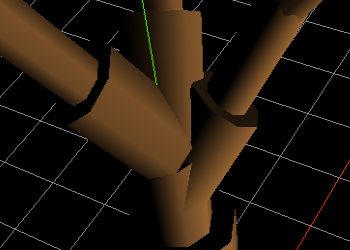
\includegraphics{fig/pseudotri}
            \caption[Pseudo-Trijunction]{The result of a pseudo-trijunction production}
            \label{fig:fig/pseudotri}

        \end{figure}
    \end{itemize}

            \subsubsection{Gaussian Density Management}
    \tab A commonly measured property of forests are the density of tree growth. As larger trees
tend to block sunlight from trees growing beneath them, in general, the older a forest is, the
further spaced its trees. Furthermore, as there is a "sweet spot" of growth away from an older tree
where light isn't blocked and roots aren't in conflict over nutrients in the soil, trees,
especially of a similar age, tend to be spaced fairly evenly. To model this, a algorithm that
roughly and indeterministically manages density is preferred. The algorithm implemented uses a
proximity detection algorithm\cite{kramii14} with the central limit theorem to filter out trees
that are packed too densely. The algorithm is as follows:
    \begin{alltt}
Gaussian-Density-Management(density)
    // Spam step
    Plant at a random location a number of trees that, given the size of the terrain,
        results in double the desired density

    // Proximity detection step
    Create a grid where each square is half the distance between trees, calculated
        from the density
    Seed grid with first tree by mapping the tree's location to the grid and adding
        it to that spot
    For every subsequent tree \(t_{dest}\),
        Map tree location to grid
        If there are any trees mapped to that location or any of its compass neighbors,
            For each neighboring tree \(t_{src}\),
                Calculate the Euclidean distance between \(t_{src}\) and \(t_{dest}\)
                Construct a pair of \(t_{src}\) and \(t_{dest}\), including the calculated
                    distance
                Add pair to a list of pairs

    // Filter step
    For each pair in the pair list
        MAP DISTANCE TO NORMAL CURVE TO GET PROBABILITY??
        FILTER USING THAT PROBABILITY??
    \end{alltt}

            \subsubsection{Gradation Detection}
            \subsubsection{Local and Global Tropism}

    \section{Implementation}
        \subsection{Top Level}

        \subsection{Terrain Implementation}
            \subsection{terrain\_gen.js}
        \subsection{Tree Implementation}
    \tab The creation of a tree begins by creating a rule set for the L-System. A few of these are
defined in \verb|./js/app/lsys_rules.js|, which can be used as an example for users wishing to
create their own L-Systems. This rule set is used to create an L-System object, which will be used
to generate the tree's geometry. A turtle must also be constructed, and must be given a set of
three.js objects in order to draw to the HTML5 canvas. Then, by calling the L-System object's
\verb|build()| method, the L-System will recursively construct a tree, storing it in its own
\verb|property| public variable. This is then passed into the turtle object's \verb|run()| method,
which will draw the constructed L-System as a single hierarchical object onto the HTML5 canvas.

            \subsubsection{turtle\_graphics.js}
    \tab The turtle graphics module consists of a turtle object, \verb|Turtle|, a set of turtle
commands to control drawing, and a \verb|run| method, which, given a list of turtle commands,
executes them in order from the current position.
\begin{itemize}
    \item \verb|Turtle(scene, material, radius)|: Turtle object constructor. Creates the turtle
drawer, initializing it at the world origin oriented in the $+z$ direction. Turtle properties
are as follows:
    \begin{enumerate}
        \item \verb|rate|: Defaults to 1. Rate at which turtle travels when moving forward,
    multiplied by the forward command's \verb|time| parameter to get the total distance traveled.
        \item \verb|width|: "Width" of the drawn line. Defaults to 0.25, can be passed in as an
    argument. Actual value is the radius of the cylinder primitive created by the turtle.
        \item \verb|scene|: Three.js scene. Must be passed in. Graphics drawn in \verb|run()| are
    added to this as a single, hierarchical object.
        \item \verb|material|: Three.js material. Must be passed in. Defines the material of the
    drawn cylinder lines.
    \end{enumerate}

    \item Turtle commands: The turtle commands (\verb|_F()|, \verb|_f()|, \verb|_pitch()|,
\verb|_yaw()|, \verb|_roll()|, \verb|_push()|, \verb|_pop()|, and \verb|_set()|) are all methods
that specify commands to some turtle object. To use, they are attached to a \verb|Turtle.Action|
object along with the value of their argument, and then passed as a list as the argument to
\verb|run()|. Each one specifies a action relative to the turtle drawer's current position and
orientation. Details of the actions are given in table 1. In general, the rotation actions work by
multiplying a specific rotation matrix to the turtle object's internal orientation matrix. The use
of a rotation matrix allows for relative transforms, as opposed to Euler coordinates, which require
specific ordering of rotations which can lead to errors. The forward movement controls drawing; it
does this by creating a cylinder of the current width and given distance (the actual given is a
time parameter, which is multiplied by the turtle's \verb|rate| to get the cylinder's length) and
moving it such that it begins at the turtle's starting position and is oriented in the same
direction of the turtle. Then, the turtle's position is incremented by the given distance.
\verb|_push()| and \verb|_pop()| save the turtle's state in a basic object and store or retrieve it
from an internal stack.

    \item \verb|run()|: The run commands executes a given turtle string. Looping through the string
in order, it run's the function's built-in \verb|call()| function, specifying \verb|this| as the
calling object and \verb|Turtle.Action.args| as the arguments. This binds the current turtle object
to the action, allowing the turtle command to affect the turtle object's internal variables.

\end{itemize}
            \subsubsection{lsys.js}
    \tab \verb|lsys.js| gives the object used to describe and create an L-System of arbitrary
productions and rule set. Relevant object, including \verb|LSystem.Production| and
\verb|LSystem.RuleSet|, are defined, and the engine to run recursion to a specific depth is
included in a method of the base \verb|LSystem| object. The L-System requires both a rule set and
an initial value to run, both of which are described below.

\begin{itemize}
    \item \verb|LSystem|: Object containing the L-System and it's rule set. The only argument is
\verb|rule_table|, the rule set for the L-System.
    \item \verb|LSystem.Production|: Object containing production information. Productions, with
the added information of their rule sets, represent a specific type of growth, but are not actually
drawn by the turtle graphics wrapper. Production arguments are as follows:
    \begin{enumerate}
        \item \verb|id|: ID of the production, similar to function name. For example, in the
production A(1,4), the id is "A".
        \item \verb|args|: List of argument values. This is only assigned for initial values; the
\verb|inject| function is used to dynamically assign these values, as the resultant value is
usually some function of the previous value, defined in the rule set.
        \item \verb|inject_args|: Function used to dynamically assign arguments from within the
rule set. Arguments after the replacement step are usually a function of their previous values;
the width of branches, for example, might decrease by a constant scale at each level of branching.
The function must take \verb|args|, the previous production's arguments, and \verb|consts|, a
dictionary of constants defined in the rule set. It must then assign \verb|this.args| to a list of
the argument values.

    \end{enumerate}
    \item \verb|LSystem.RuleSet| and \verb|LSystem.Rule|: \verb|RuleSet| and \verb|Rule| are used
to define the logic of the L-System. \verb|RuleSet| describes the entire rule system, whereas Rule
defines a single rule for a specific production and condition. The arguments for the \verb|RuleSet|
constructor are as follows:
    \begin{enumerate}
        \item \verb|consts|: Dictionary of defined constants, such as width reduction ratios, used
    in calculating the argument values at replacement.
        \item \verb|initial|: Initial production list values for the system.
        \item \verb|rules|: List of rule objects for this system.
See \verb|lsys_rule.js| and its below explanation for more details on \verb|LSystem.RuleSet|
construction.

    \end{enumerate}
The arguments for the \verb|Rule| constructor are as follows:
    \begin{enumerate}
        \item \verb|id|: ID corresponding to the production this rule affects.
        \item \verb|condition|: Condition function to the parametric term. Function takes as
    argument the production object and returns a boolean. Allows the rule to match on the
    value of the production's parameter. 
        \item \verb|output|: List of production and turtle action objects to replace the matched
    production with upon recursion. 

    \end{enumerate}
More details about the construction of a \verb|RuleSet| can be seen in the documentation for
\verb|lsys_rule.js|.

    \item \verb|build()|: Launcher function for the recursive L-System construction. Calls internal
recursion function on each element in the initial system; thus, it requires that the \verb|system|
variable is set to a list of initial values. The internal recursion runs for a single object in the
system list, matching it to the rule set and replacing it with the appropriate output string. It
then recursively calls itself on each element of the output array, to a specified \verb|MAX_DEPTH|
value. Optional argument \verb|debug| is a boolean that toggles printing of the constructed system
after construction.

    \item \verb|checkRule()|: Function that checks a given element of the system against the
system's rule set, returning the appropriate output. Does a linear search through the list of
rules, halting when a match occurs. Matches require that both the rule id and the production id
match, as well as the rule's \verb|condition| function returning a \verb|true|. The rule's output
is then cloned to avoid problems with Javascript's singleton objects affecting subsequent
production values. The arguments are then injected using the production's provided
\verb|inject_args| function, which allows dynamic evaluation of the arguments based on the
previous production. The output is then returned. If no match is found, the initial production is
returned unchanged.

    \item \verb|printSystem()|: Used for debugging. Pretty prints the current value of the
L-System's \verb|system| variable, in form \verb|id(args...)|. Used when the \verb|debug| flag is
turned on in \verb|build()|.

\end{itemize}

            \subsubsection{lsys\_rule.js}
    \tab \verb|lsys_rule.js| provides a convenient package of L-System rules used in \emph{The
Algorithmic Beauty of Plants}. The rules found in it are used to create the trees in the final
Garden of Eden project, but can also serve as examples to users wishing to generate their own
L-Systems. The structure for a rule set is given in the above description of
\verb|LSystem.RuleSet|.
    \begin{itemize}
        \item \verb|HondaTree|: Creates an object that inherits from \verb|LSystem.RuleSet|.
Description of a Honda L-System comes from \emph{SOURCE WEE}. The tree is of a constant height, but
branches with increasing detail at higher levels of recursion. Defined constants allow for a
decent amount of variation on what is otherwise a visually highly symmetrical tree.

        \item \verb|TernaryTree|: Creates an object that inherits from \verb|LSystem.RuleSet|.
Description of a Ternary L-System comes from \emph{SOURCE WEE}. By using L-System rules that match
to turtle commands, this tree actually grows both larger and more detailed at higher levels of
recursion, which more closely resembles the growth of a tree. There is only one branching rule,
which erroneously uses a trijunction at each branching node. The generated tree is visually quite
complex, but has some symmetrical artefacts visible from specific angles. Varying constants allows
for a large amount of variation on this tree structure.

    \end{itemize}

    \section{Runtime} % Why I want it fast, how fast is it
        \subsection{LList Algorithm}
            \subsubsection{Profile}
            \subsubsection{Asymptotic Behavior}
        \subsection{Tree Search Algorithm}
            \subsubsection{Profile}
            \subsubsection{Asymptotic Behavior}
        \subsection{Three.js Considerations}

    % ADD what I learned?

    \nocite{*}
    \bibliographystyle{plain} % abbrev?
    % dblpp
    \bibliography{refs}
\end{document}
